\chapter{MODULES FOR DIRTY PAPER CODING}
\label{chap:dpc-modules}

%%%%%%%%%%%%%%%%%%%%%%%%%%%%%%%%%%%%%%%%%%%%%%%%%%%%%%%%%%%%%%%%%%%%%%%%%%%%%%%

\section{Log Likelihood Ratio computation}

There is a requirement for the computation of log-likelihood ratios prior to
decoding the constellation symbols. Furthermore, this log-likelihood ratio is
to be computed on a repeated constellation.

The reason for this is that while transmitting symbols (from a base station to
a user in a 2-user system) in the DPC framework, interference from user 2 has
to be pre-subtracted from the constellation symbol being transmitted for user
1. During this process, it is possible that the symbol that is finally to be
transmitted lies outside of the constellation boundary. In such a situation,
the symbol in question is removed and reintroduced on the other side of the
constellation. The operation can be likened to a modulo operation, pulling
symbols outside of an interval back into the interval by repeatedly subtracting
the interval size.

On the receiver side, for the computation of LLRs, it is essential for
correctness to consider the possibility that a symbol might actually have come
from an out-of constellation point, or effectively from the other side of the
constellation. For the purpose of LLR computation, therefore, we can assume
that the symbol came from a repeated grid of the constellation.

This has currently been implemented only for a repeated 256-QAM constellation.

\subsection{Approximation of LLR}

The likelihood ratio is defined for each received bit as the ratio of the
probability of the corresponding transmitted bit being a 1 to to that of it
being a 0. This probability is computed for a given known noise variance, which
must be estimated beforehand.

In a 256-QAM constellation, the received constellation symbol could have come
from any of the 256 constellation points. Each constellation point encodes 8
bits. So from one received 256-QAM constellation point, we get 8 LLR values. At
any given bit position, half the constellation points will correspond to 0 and
the other half to 1. For computing the exact LLR value, we consider the
probability of the bit having come from each of these constellation symbols.

Let $s_i$ be the transmitted constellation points and $r$ be the received
complex vector. We wish to compute the LLR for a given bit (position) $b$. Let
$S^0$ be the set of indices $i$ for which $s_i$ has a 0 at bit position $b$,
and $S^1$ be the set of indices for which $s_i$ has a 1 at bit position $b$.
Then, the LLR for bit $b$ of the received vector $r$ is
\begin{equation}
	\text{LLR}(b) = \text{log} \left (
		\frac{ \sum_{i \in S^0}{e^{- |s_i - r|^2 / (2 \sigma^2)}} }
		     { \sum_{i \in S^1}{e^{- |s_i - r|^2 / (2 \sigma^2)}} }
		\right )
\end{equation}
where $\sigma^2$ is the noise variance.

To compute the LLR for each bit thus becomes very expensive, because it
involves 256 exponentiation operations. Since these LLR values are used only as
guides in the LDPC decoder, we do not need the exact LLR values. It is
sufficient to have good approximations of the same.

To this end, we neglect all terms except the dominant one in the numerator and
denominator of the likelihood ratio expression. That is to say, we redefine the
likelihood ratio as the ratio of the probability that the given received bit is
a 1, given that it came from the nearest constellation point having a 1 at the
corresponding bit location, to the probability that the given received bit is a
0, given that it came from the nearest constellation point having a 0 at the
corresponding bit location.
\begin{align}
	\text{LLR}_{\text{approx}}(b) &= \text{log} \left (
		\frac{ e^{- |s_{i^*_0} - r|^2 / (2 \sigma^2)} }
		     { e^{- |s_{i^*_1} - r|^2 / (2 \sigma^2)} }
		\right ) \\
		&= \frac{|s_{i^*_1} - r|^2 - |s_{i^*_0} - r|^2}{2 \sigma^2}
\end{align}
where $i^*_0$ corresponds to the nearest constellation point with index in
$S^0$ and $i^*_1$ corresponds to the nearest constellation point with index in
$S^1$.

\subsection{Computation of the approximate LLR}

In order to compute the approximate LLR for a bit, we need only the distance to
the constellation points corresponding to the nearest 0 and the nearest 1 for
that bit. To simplify our approach, we rely on the fact that \emph{the
constellation points corresponding to the nearest 0 and the nearest 1 are the
same (constant) for all points (all possible receive vectors) within the
decision region of each transmitted constellation point}.

In other words, we can precompute the constellation points corresponding to the
nearest 0 and the nearest 1 for each transmitted constellation point and store
these values in a table.  Then, we only need to find out the nearest
constellation point corresponding to a receive vector. This will tell us the
nearest 0 and the nearest 1 corresponding to a receive vector. Subtracting the
squares of the distances gives us the required LLR value.

\subsection{Nearest constellation point in a repeated constellation}

In order to compute the approximate LLR, we need to find the nearest
constellation point to the received vector. This is equivalent to the operation
of slicing, or locating which decision region the given receive vector lies
within. The only difference is that we need to do this in a repeated
constellation setting. This, in fact, makes our job a whole lot easier, because
it enables us to use floor and modulo operations.

\begin{figure}[h]
	\centering
	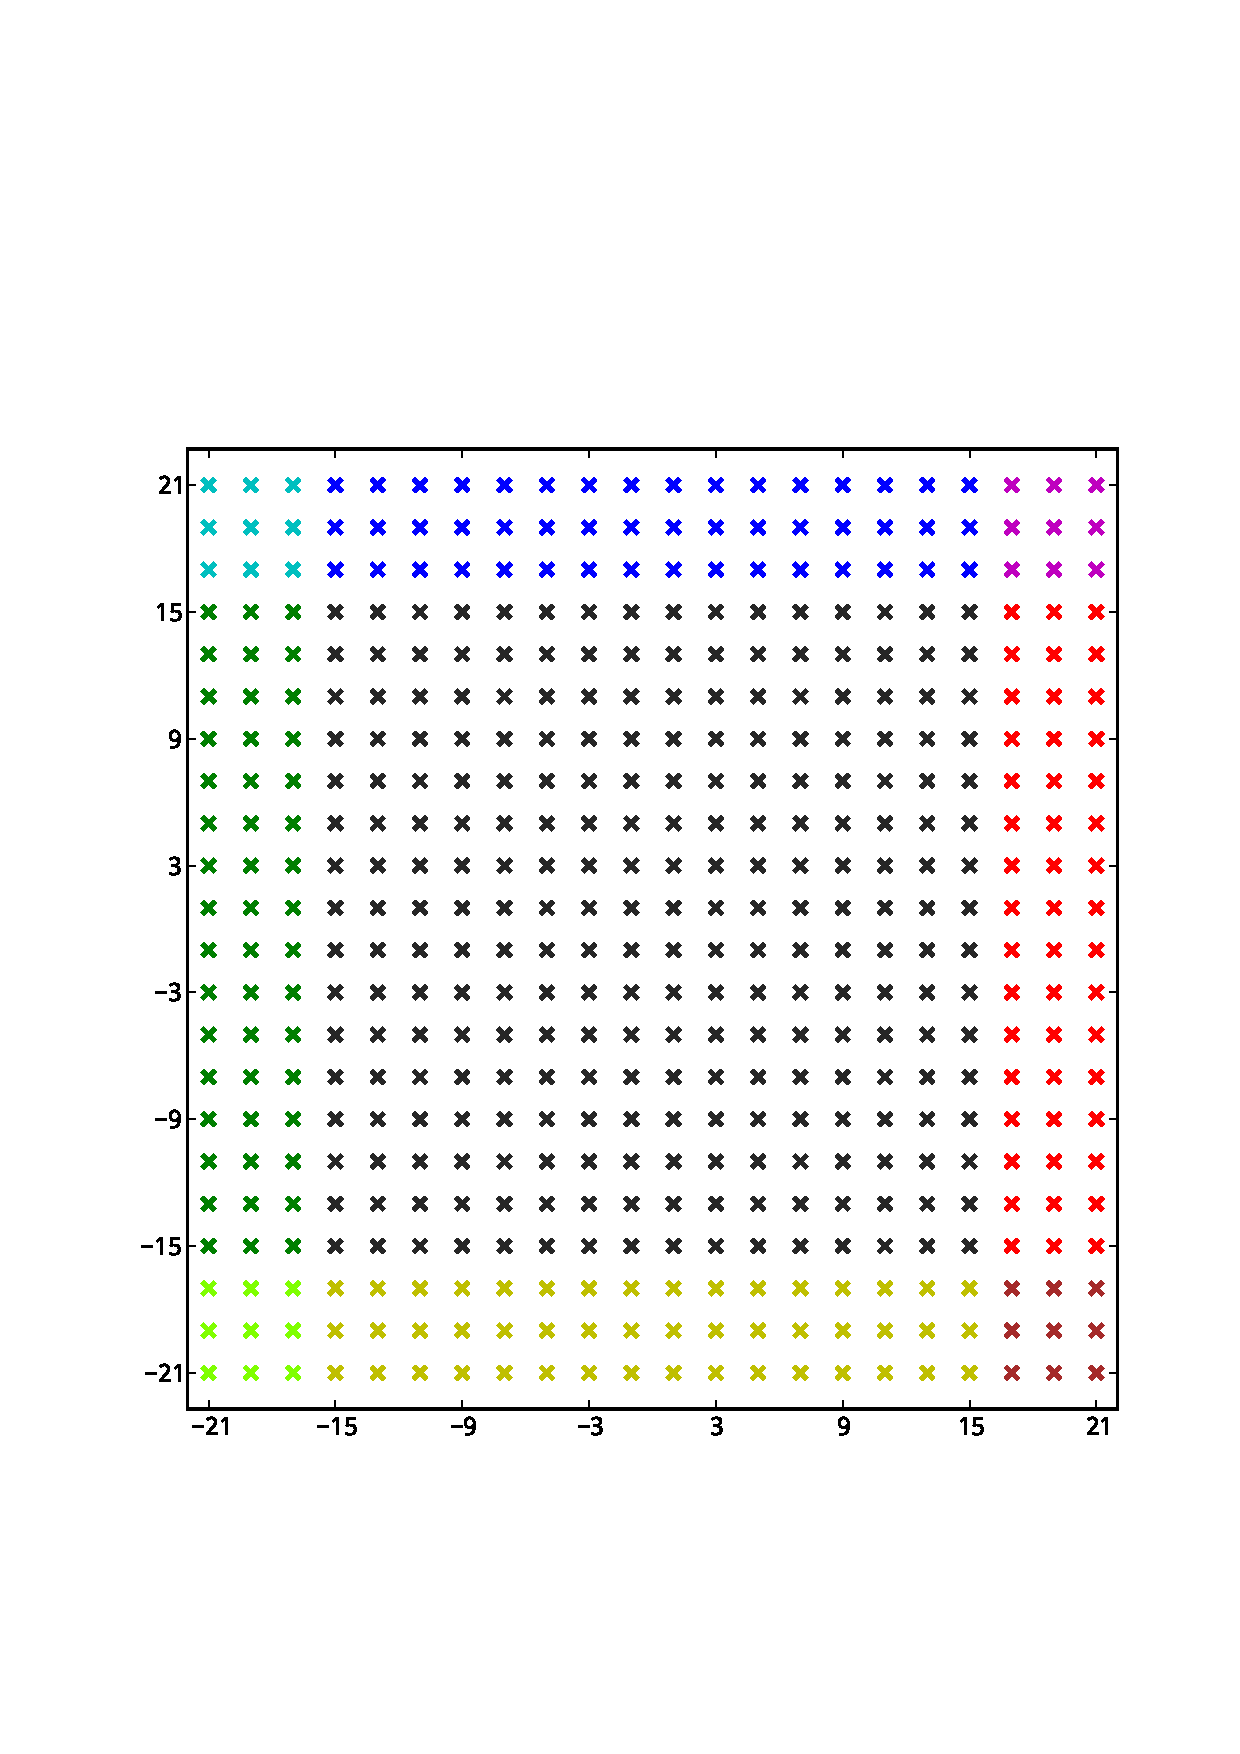
\includegraphics[width=0.8\textwidth]{256-qam-reptd-constln}
	\caption{Repeated 256-QAM constellation, prior to normalization. The
	         primary constellation is black, while its repetitions are coloured
	         variously.}
	\label{fig:256-qam-reptd}
\end{figure}

Consider the canonical 256-QAM constellation where constellation points are
located at odd points on the grid, from $-15$ to $+15$, on both real and
imaginary axes. On top of this, we have repetitions, so that the same
constellation is also present from $-47-15j$ to $-17+15j$ (left-bottom and
right-top corners of the constellation rectangle being used to denote
boundaries) on the left, from $-15+17j$ to $15+47j$ on the top, and so on in
all other directions (refer figure~\ref{fig:256-qam-reptd}).

Note that constellation points on $x=-17$ encode the same 8 bits as
constellation points on $x=+15$, and so on. This is the idea behind the
\emph{`modulo'} or the \emph{`repetition'}. This enables us to do the following
for slicing: we scale and translate the decision boundaries of the
constellation to the points of discontinuity of the floor function, and use the
floor function to achieve slicing. Following this, we use a modulo operation to
bring all repeated constellation points back into the primary constellation.

\begin{lstlisting}
	double x = creal(received_symbol);
	double y = cimag(received_symbol);
	// Move the received point back into the primary constellation
	x -= 32 * floor((x+16) / 32);
	y -= 32 * floor((y+16) / 32);
	// Find the index of the nearest constellation point
	int x_index = (int)(floor(x / 2) + 8);
	int y_index = (int)(floor(y / 2) + 8);
\end{lstlisting}

%%%%%%%%%%%%%%%%%%%%%%%%%%%%%%%%%%%%%%%%%%%%%%%%%%%%%%%%%%%%%%%%%%%%%%%%%%%%%%%

\section{Viterbi algorithm for Joint Trellis Shaping}

Joint Trellis shaping is aimed at minimizing the transmitted constellation
energy over a large number of constellation symbols. In order to do this with
greater ease, we use an almost-gray mapping scheme for the constellation.

The mapping for 256-QAM is based off the mapping for 16-PAM. The first four
bits are mapped using a 16-PAM constellation to get the real part of the
256-QAM constellation point. Similarly, the next four bits are used to get the
imaginary part.

%TODO: Insert 16-PAM constellation.

The 16-PAM constellation used is almost-Gray coded. Notice that the last three
bits read the same when sarting at $-15$ and going right, and when starting at
$+1$ and going right. The first bit, i.e.\ the sign bit, can therefore be used
to position the constellation point towards the centre of the constellation
(with lower energy) or towards the edge of the constellation (with higher
energy).

The point of trellis shaping is to choose sign bits in such a way as to
minimize the overall constellation energy, averaged over many transmitted
symbols. In the case of DPC, we need to perform joint trellis shaping, wherein
we minimize the overall average constellation energy of two users. To achieve
this the optimal way, we make use of the Viterbi algorithm.

\subsection{Shaping using the trellis}

The Viterbi algorithm is used to find the optimal sequence of signed bits to
minimize the overall energy of the transmitted symbols. Different choices of
signed bits make different paths in the trellis. The branch metric corresponds
to the energy of the constellation point generated by a certain choice of sign
bits. Thus, by finding the optimal path, we minimize the overall transmit
energy.

\subsection{Implementing the Viterbi algorithm}

In the Viterbi algorithm, edge weights (or the branch metrics) denote the
`cost' of choosing a certain path and node weights denote the accumulated
minimum cost of reaching that particular node.

We start by assigning a node weight of zero to the left-most states in the
trellis. Following this, at `time step', we need to compute the edge weights.
Given a set of input bits, we need to evaluate all possible choices of sign
bits. Each edge's weight is then the transmitted energy of the corresponding
constellation point that results from choosing that particular sign bit.Next,
we need to update the node weights of the next time step. This is done by
choosing, for each node, an input edge, which yields the least cost after
adding its branch metric with the corresponding source node's weight. A summary
of this algorithm in pseudocode is presented in algorithm~\ref{alg:viterbi}.

\begin{algorithm}[h]
	\SetKwData{Edge}{edge} \SetKwData{ToNode}{to\_node} \SetKwData{FromNode}{from\_node} \SetKwData{StateDiagram}{state\_diagram} \SetKwData{Weight}{weight}
	\SetKwData{MinNode}{min\_node} \SetKwData{PrevNode}{prev\_node} \SetKwData{Path}{path} \SetKwData{Node}{node}
	\SetKwFunction{Min}{Min} \SetKwFunction{Compute}{Compute}
	\SetKwInOut{Input}{input} \SetKwInOut{Output}{output}

	\Input{\StateDiagram;$\;$\emph{input bits for \Edge.\Weight computation}}
	\Output{\Path}
	\BlankLine
	\emph{initialize start node weights to $0$}\;
	\emph{initialize all other node weights to $\infty$}\;
	\ForAll{time steps} {
		\ForEach{\Edge in \StateDiagram} {
			\Compute{\Edge.\Weight}\;
			\If{\Edge.\ToNode.\Weight $>$ \Edge.\FromNode.\Weight $+$ \Edge.\Weight} {
				\Edge.\ToNode.\Weight $\leftarrow$ \Edge.\FromNode.\Weight $+$ \Edge.\Weight\;
				\Edge.\ToNode.\PrevNode $\leftarrow$ \Edge.\FromNode\;
			}
		}
	}
	\MinNode $\leftarrow$ \Min{final nodes}\;
	\Node $\leftarrow$ \MinNode\;
	\While{\Node not in start nodes} {
		\Path $\leftarrow$ \Node\;
		\Node $\leftarrow$ \Node.\PrevNode\;
	}
	\Return \Path\;
	\caption{The Viterbi algorithm}
	\label{alg:viterbi}
\end{algorithm}
